\subsection{Optimizations}
\label{subsec:cuda:load}

\todorev{Last revised on Sun, July 1 at 00:10 by pfac}

One of the first optimizations performed comes from a simplification already explained in \cref{sec:seq:optimizations}.
The initial implementation, like the CPU versions, relied on a reduction to compute the maximum velocity after each iteration.
The reduction used was based on the most optimized implementation provided in the NVidia samples, and is, according to the author, one of the most optimized CUDA reductions.

But the simplification of moving the maximum velocity computation to preprocessing stage did not rely only on the reduction, as that was only the final step of the computation.
There was also added workload to the \computeflux kernel, which had to compute the velocity for each edge. More than the amount of operations, this had a considerable impact on the amount of registers used by the kernel, allowing for more threads to be spawned without having register spilling, and it was noted that after its removal.

\subsubsection{Second Phase}
\label{subsubsec:cuda:load:second}

On the second phase of the development of a CUDA implementation, more attention was given to the individual performance of the kernels.
Several experiments were performed with different kernel implementations, in order to test different approaches to eliminate memory accesses and reduce or eliminate divergent branches.

While this provided small improvements to kernel execution time (consequently decreasing the main loop time considerably) the better speedup was achieved after a division operation was removed from \update, which computed a ratio between the length of an edge and the area of a cell.
This was achieved by precomputing a matrix with the value of the ratio in the preprocessing stage.
This required a considerable amount of additional memory to be used on the GPU, but since the problem is not bound by total size (largest test case used consisted of less than 100MB) and division operations are very costly to a GPU, this showed large improvements for the \update kernel.

%\begin{figure}[!htp]
%	\begin{subfigure}[b]{\columnwidth}
%		\centerign
%		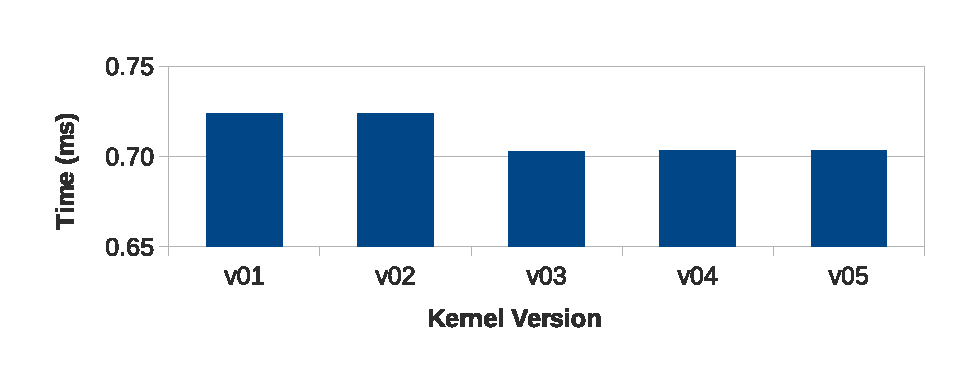
\includegraphics[width=\columnwidth]{graph_compute_flux}
%		\caption{\computeflux}
%		\label{fig:time_computeflux}
%	\end{subfigure}
%	\begin{subfigure}[b]{\columnwidth}
%		\centering
%		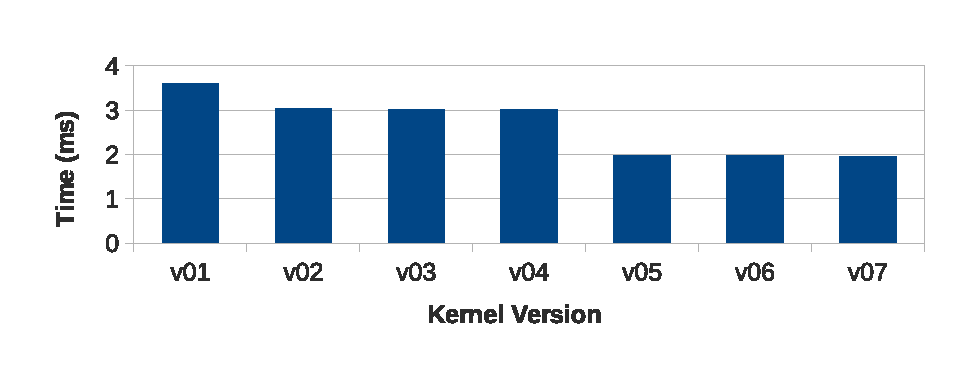
\includegraphics[width=\columnwidth]{graph_update}
%		\caption{\update}
%		\label{fig:time_update}
%	\end{subfigure}

\begin{table}
	\centering
	\begin{tabular}{r|cc|c}
						&	Initial	&	Optimal	&	Speedup	\\ \hline
		\computeflux	&	0.72	&	0.7		&	\textbf{1.03}	\\
		\update			&	3.60	&	1.96	&	\textbf{1.84}	\\ \hline
	\end{tabular}
	\caption{Comparison of first and last kernel implementations. Times are in ms.}
	\label{tab:kernel_speedups}
\end{table}

Times shown in \cref{tab:kernel_speedups} were measured using the CUDA Events API, which allows measurements of GPU events, excluding the callback overhead of issuing a kernel call. That, along with the fact that both kernels have considerably short and simple code, explains the low times, even for the initial versions.
Even so, the removal of the division operation, along with other smaller tweaks through branchless operations, allowed the execution time of the \update kernel to be almost halved.

Due to the low precision of the measurements when compared to the small execution time of the kernels\footnote{CUDA Events API claims a precision of only 0.5 ms}, no immediate changes can be seen between some of the versions. However, since later kernels are the result of aggregating most optimizations from previous versions, intermediate results are still influent.
